\documentclass{article}
\usepackage[utf8]{inputenc}
\usepackage[margin=1in]{geometry}
\usepackage{amsmath}
\usepackage{amsthm}
% Package for making turing machine diagrams %
\usepackage{tikz}
\usetikzlibrary{chains,fit,shapes}
% Packages for algorithms %
\usepackage{algorithm}
\usepackage{algorithmic}
% Package which has the nice looking empty set symbol (\varnothing)
\usepackage{amssymb}
% Package with the ceiling function
%\usepackage{mathtools}
%\DeclarePairedDelimiter{\ceil}{\lceil}{\rceil}
\usepackage{braket}
\usepackage{amsmath} 
\usepackage{amsfonts}
\usepackage{amssymb}
\usepackage{comment}
\usepackage{mathtools}
\DeclarePairedDelimiter{\ceil}{\lceil}{\rceil}
\usepackage{bm}

\usepackage{biblatex}
\addbibresource{bibliography.bib}

% Makes table of contents links clickable in pdf readers
\usepackage[colorlinks=true, linkcolor=blue, urlcolor=blue, citecolor=blue, breaklinks=true]{hyperref}

\theoremstyle{definition}
\newtheorem{definition}{Definition}[section]
\newtheorem{problem}{Problem}

\theoremstyle{plain}
\newtheorem{example}{Example}[section]
\newtheorem{exercise}{Exercise}[section]

\theoremstyle{plain}
\newtheorem{fact}{Fact}[section]
\newtheorem{lemma}{Lemma}[section]
\newtheorem{theorem}{Theorem}[section]
\newtheorem{corollary}{Corollary}[section]
\newtheorem{claim}{Claim}[section]

\title{Reachability, Complexity, and the Limits of Conway's Game of Life}
\author{Sebastian Pucher \& Adam Gohain}

\begin{document}

\maketitle

\tableofcontents

\newpage

\section{Introduction: Can Life be Simulated?}
  \textit{    That is the question, isn't it.} For centuries, mathematicians, philosophers, artists, and computer scientists, have spent their lives trying to uncover what it means to truly be alive. Many come together, often crossing their respective disciplines to construct answers to these larger, often existential questions. Even today, humanity has continued to develop complicated technology in hopes of understanding more about life, how it can be studied, or even how it could possibly be synthesized.

\

\textit{What is life?} Back in 1940, John Von Neumann and Stanislaw Ulam set out to prove an answer to this very question. Von Neumann was an American Mathematician whose research focused on self-replicating systems and cellular automata. Alongside his colleague Ulam, who worked together with Von Neumann on the Manhattan Project, they proposed a simple discrete game that replicated life. Their mathematical model consisted of a two-dimensional grid of square cells, where the state of the next generation of cells would depend on the interaction between living cells and their neighbors \cite{Beginning_Life_2006}. They called it \textit{The Universal Constructor} which produced fascinating properties of time and space usage \cite{Freitas_2004}.

\

Not long after their proposal, a British Mathematician known as John Conway extended upon Ulam and Von Neumann’s research to fabricate an instance of their Universal Constructor that better replicated Alan Turing’s “universal computer”. By experimenting with different rules and states between neighboring automata, Conway was able to simplify the model into a game that was only composed of only a few basic rules \cite{Beginning_Life_2006}. [see section (CITE SECTION)]. 

\

Shortly after, in 1970, the \textit{Scientific American} published an article articulating how to play the game which resulted in the greatest number of letters reactions from readers at that time \cite{Izhikevich_Conway_Seth}. In the paper, Conway proposed that no initial pattern could grow without limit, and offered fifty dollars to the first person who could disprove him by the end of the year \cite{math-games}. This catalyzed immense popularity in the game, and set forth the many mathematical discoveries that have now been proven about the game, such as its undecidable nature (see section (CITE SECTION)), and recurring patterns(see section).


\textbf{Going to add a nice image here}

\subsection{The Game}
Similar to how Alan Turing proposed models of computational thinking prior to modern day computers, Conway's Game of Life started as a simple mathematical idea that was “played” on chalkboards and Go boards \cite{Izhikevich_Conway_Seth}. Here are the rules, and how to play: 

\

\textbf{Rules \& Properties: }
\begin{enumerate}

  \item \textbf{Domain: }\\ The automata in the game interact within an \textit{infinite} two-dimensional grid of cells. Every cell has eight neighbors \cite{Izhikevich_Conway_Seth}[figure x].

  \item \textbf{States: }\\ Each automata is represented independently by a single cell which can be either \textit{alive} or \textit{dead}.

  \item \textbf{Initial Configuration: } \\ The beginning set of live or dead cells is determined or "seeded" by the player prior to any evolution.

  \item \textbf{Evolution: } \\ The following rules are applied to all cells simultaneously in fixed time intervals called \textit{generations} \cite{Bontes2019}.

  \item \textbf{Birth: } \\ A new cell is born at generation $t + 1$ when its state is currently \textit{dead} and has exactly three lives neighbors (reproduction) \cite{Bontes2019}.

  \item \textbf{Death: } \\ Any currently living cell will die at generation $t + 1$ if it has less than 2 live neighbors (underpopulation) or more than three live neighbors (overpopulation) \cite{Bontes2019}.

  \item \textbf{Persistence: } \\ Any live cell will persist at $t + 1$ if it has two or three live neighbors at generation $t$ \cite{Izhikevich_Conway_Seth}.
\end{enumerate}

It’s important to note that Conway’s Game of Life is not a game of how we traditionally think of games. There’s no objective, or winning or losing. They’re aren’t even any players – it is known to be a zero player game \cite{Beginning_Life_2006}. As technology advanced, Conway’s Game of Life proved to be well-suited for implementation on computers. Today, the game has been optimized to explore the many unresolved problems and complexity the game poses. 

\subsection{So... What's the Big Deal?}

At first glance, Conway’s game appears to be a simple simulation of life based on just a few rules. However, beneath the surface, the Game of Life hides mathematical complexities that have perplexed many since its proposal way back in 1970. Many of its implications stem from the fact that the game is Turing Complete. Entire self-replicating machines, digital circuits, and unique patterns have been discovered and studied within the properties of the game. In fact, new behaviors are still being uncovered today. 

\ 

\textbf{Proposal}: The purpose of this paper is to both synthesize concrete theoretical mathematics from Complexity Theory into a specific instance of Conway's game of life. More specifically, the paper will be divided into two parts. The first pertaining to the Pattern reachability question, and the second pertaining to Undecidability and Turing Completeness in Conway’s Game of Life. 


\section{Definitions, Theorems, and other Important Terminology}
\begin{enumerate}
  \item[] \textbf{GOALS FOR SUB SECT}
  \item Explain the common patters / life forms that can be found in the game
  \item Explain the three patterns we will be examining (Still life, ociliator, and spaceship)
  \item Add images to these 
  \item Explain other relevant mathematical terminology / information that's worth introducing 

\end{enumerate}

\subsection{What about Complexity?}
\begin{enumerate}
  \item[] \textbf{GOALS FOR SUB SECT}
  \item More of an intro sub section connecting the game to complexity analysis  
  \item This is where we'll define important compelexity classes like NP
  \item outline any other important info we want to outline before getting into more gritty / mathy stuff

\end{enumerate}

\section{Reaches-Configuration}

\subsection{Still life Analysis}
\begin{enumerate}
  \item[] \textbf{GOALS FOR SECTION}
\end{enumerate}

\subsection{Oscillator Analysis}
\begin{enumerate}
  \item[] \textbf{GOALS FOR SECTION}
\end{enumerate}

\subsection{Spaceship Analysis}
\begin{enumerate}
  \item[] \textbf{GOALS FOR SECTION}
\end{enumerate}

\section{What can be computed/decided in Conway’s Game of Life?}

% TODO: add personality..improve flow w.r.t. now made sections
% no need to rehash turing complete
The quest to understand the limits of computation has been a central theme in computer science since its inception. Alan Turing's groundbreaking work introduced the concept of a theoretical machine, now known as the Turing machine (TM), capable of simulating any algorithm. As we talked about in class, systems that possess this capability are deemed \textit{Turing complete}, signifying they have the maximum theoretical computational power. Discovering that a system, especially one with seemingly simple rules like Conway's Game of Life, is Turing complete reveals a profound depth and complexity. It implies that the system can, in principle, compute anything that any other computer can. This section delves into the remarkable computational capabilities embedded within the evolving patterns of Conway's Game of Life, exploring how complex computational structures, including Turing machines themselves, can emerge from its basic local interactions.

In short, we'll provide an overview of how it's even possible to construct a Universal Turing machine (UTM) in Life, and why that validates it as a Turing complete model of computation.

\subsection{Gliders}

A \textit{glider} is a specific pattern in Conway's Game of Life that exhibits translational movement across the grid while undergoing periodic transformations in its structure. Formally, we define a glider as follows:

\begin{definition}[Glider]
A glider is a configuration $G$ of live cells in Conway's Game of Life such that:
\begin{enumerate}
    \item After exactly $p$ generations (where $p = 4$), the pattern transforms into a translated version of itself: $G_{t+p} = T(G_t)$, where $T$ represents a translation operation.
    \item The translation $T$ corresponds to a diagonal movement by one cell diagonally (specifically, $\pm 1$ cell horizontally and $\pm 1$ cell vertically).
    \item The pattern consists of exactly 5 live cells in each of its phase configurations.
    \item The pattern cycles through exactly 4 distinct configurations before returning to a translated version of its initial state.
\end{enumerate}
\end{definition}

As illustrated in Figure \ref{fig:glider-generations}, the glider completes a full cycle every 4 generations, moving one cell diagonally in the process. The minimal glider discovered by Conway consists of 5 live cells arranged in an asymmetric pattern that evolves through 4 distinct phases before returning to its original configuration, albeit in a new position.

\begin{figure}[H]
  \centering
  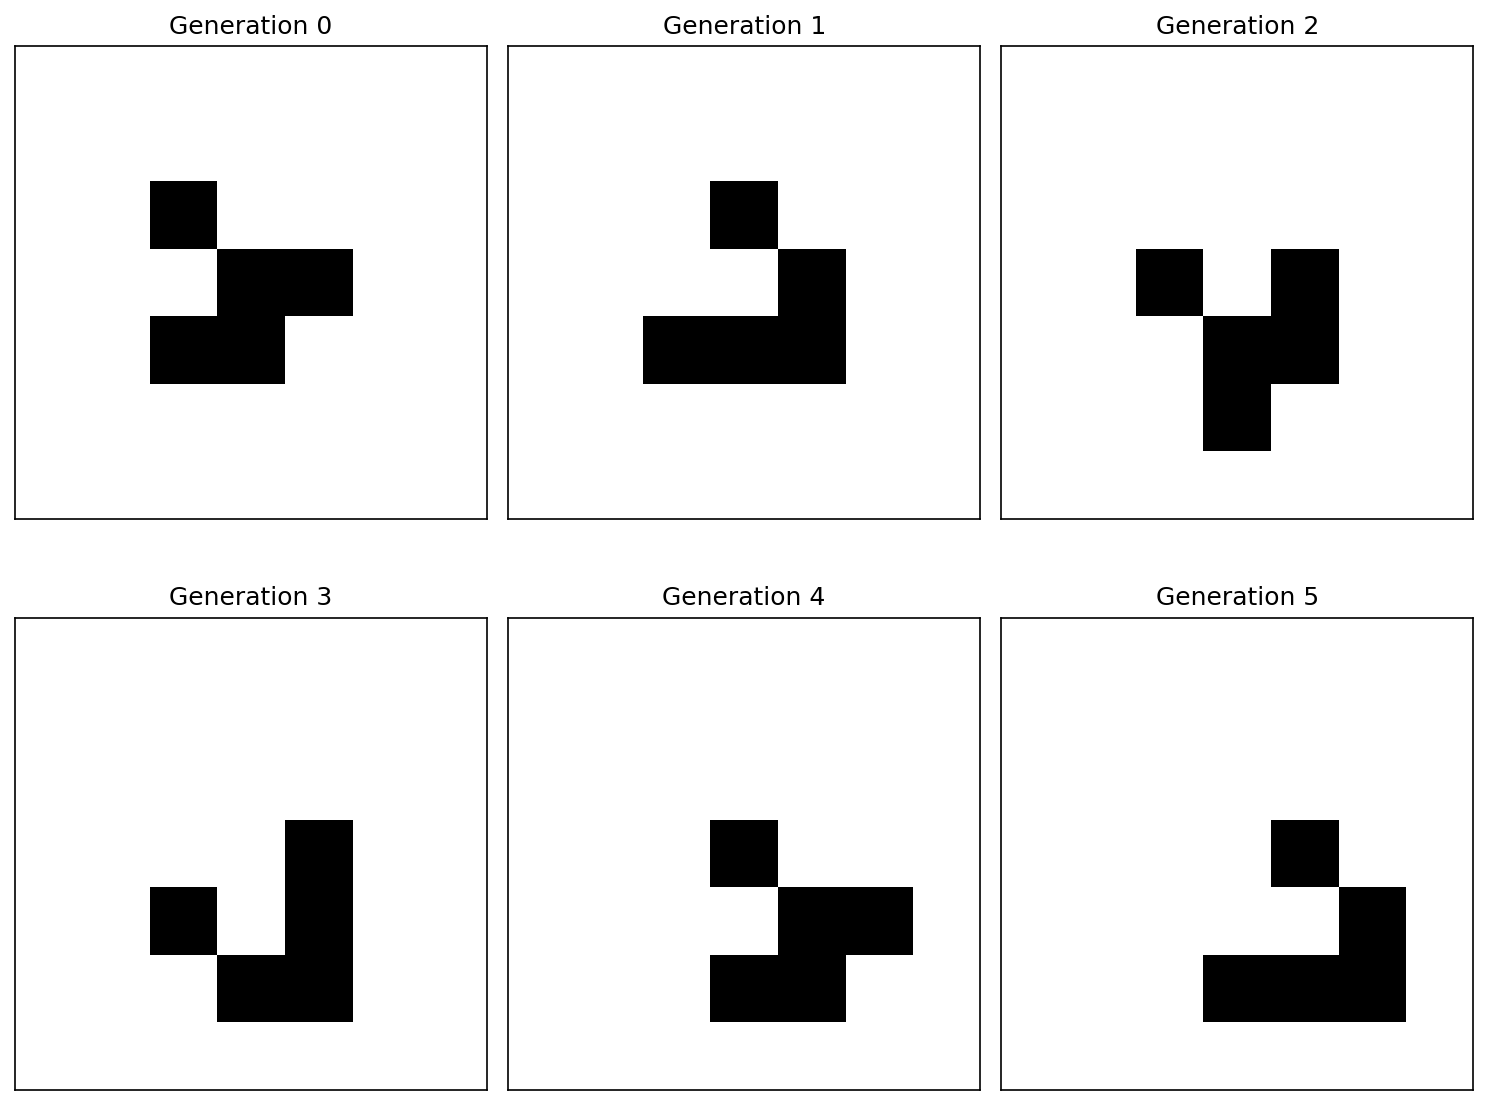
\includegraphics[width=0.8\textwidth]{figures/glider_generations_0_to_5.png}
  \caption{Evolution of a glider pattern through generations 0 to 5, demonstrating the characteristic diagonal movement and shape cycle.}
  \label{fig:glider-generations}
\end{figure}

Gliders are particularly significant in Conway's Game of Life because they serve as the fundamental mechanism for information transfer, as we'll see in the next few sections. Since they can travel arbitrarily far across the infinite grid, they effectively function as signals or "data packets" in computational constructions. In order to talk about operations on such "data" later on, we'll also need to define the following:

\begin{definition}[Glider Collision]
Let $G_1$ and $G_2$ be glider patterns with positions $P_1(t)$ and $P_2(t)$ at time $t$, where $P_i(t)$ denotes the set of coordinates of live cells comprising glider $G_i$. A glider collision occurs at time $t_c$ if there exists a time $t_c$ such that:
\begin{enumerate}
  \item For all $t < t_c$, the evolution of $G_1$ and $G_2$ proceeds independently, i.e., the state of each cell at time $t$ depends only on its own glider pattern's evolution.
  \item At time $t_c$, there exists a neighborhood $N$ such that both gliders influence the evolution of cells in $N$, formally: $\exists N \subseteq \mathbb{Z}^2$ such that $d(P_1(t_c), N) \leq 1$ and $d(P_2(t_c), N) \leq 1$, where $d$ denotes minimum Manhattan distance.
\end{enumerate}

The outcome of a collision at time $t_c+k$ (for some finite $k > 0$) can be classified as one of:
\begin{enumerate}
  \item \textit{Annihilation}: The resulting pattern $R(t_c+k)$ contains no persistent structures, i.e., $\exists t' > t_c+k$ such that $\forall t > t'$, $R(t) = \emptyset$.
  \item \textit{Reflection}: The resulting pattern contains exactly two gliders $G'_1$ and $G'_2$ with velocity vectors $v'_1$ and $v'_2$ such that $v'_i \neq v_i$ for at least one $i \in \{1,2\}$.
  \item \textit{Transformation}: The resulting pattern contains at least one glider with a velocity vector different from both $v_1$ and $v_2$, or the number of resulting gliders differs from the initial number.
  \item \textit{Creation}: The resulting pattern contains both one or more gliders and at least one persistent non-glider structure (still life or oscillator).
\end{enumerate}
\end{definition}

% figure
% make an animation for each?

\begin{definition}[Glider Gun]
A pattern $G \subseteq \mathbb{Z}^2$ is a glider gun with period $p \in \mathbb{Z}^+$ if there exists a finite core region $C \subseteq \mathbb{Z}^2$ and a sequence of configurations $(G_t)_{t=0}^{\infty}$ representing the evolution of $G$ under Conway's Game of Life rules such that:
\begin{enumerate}
  \item There exists a non-empty finite set $C \subseteq G$ such that $\forall t \geq 0$, $G_t \cap C = G_{t+p} \cap C$
  
  \item There exists a sequence of times $(t_n)_{n=1}^{\infty}$ with $t_n = np + d$ for some fixed offset $d \in \{0, 1, \ldots, p-1\}$ and a glider pattern $H$ such that:
    \begin{itemize}
      \item For each $n \geq 1$, there exists a translation vector $\vec{v}_n = n \cdot \vec{v}$ for some fixed $\vec{v} \in \mathbb{Z}^2 \setminus \{(0,0)\}$ such that $H + \vec{v}_n \subseteq G_{t_n}$
      \item For any distinct $n, m \geq 1$, the patterns $H + \vec{v}_n$ and $H + \vec{v}_m$ are disjoint
    \end{itemize}
    
  \item There exists $T \in \mathbb{Z}^+$ such that for all $n \geq 1$ and all $t \geq t_n + T$, the evolution of $H + \vec{v}_n$ proceeds independently of both the core region $C$ and all other emitted gliders
  
  \item The distance between the core region $C$ and the $n$-th emitted glider $H + \vec{v}_n$ increases without bound as $n \to \infty$
\end{enumerate}
\end{definition}

% \begin{figure}[htb]
%   \centering
%   \includegraphics[width=0.6\textwidth]{figures/gosper_glider_gun.png}
%   \caption{The Gosper glider gun, the first known pattern to produce an infinite number of moving objects. It has a period of 30 generations and emits a new glider every 30 steps.}
%   \label{fig:gosper-gun}
% \end{figure}

The discovery of the Gosper glider gun in 1970 was pivotal, as it disproved Conway's conjecture that no pattern could grow indefinitely. More importantly, the ability to generate endless streams of gliders provides the foundation for information processing (which we keep omniously alluding to!!!).




\subsection{A Turing Machine in Life}



\subsection{Constructing a Universal Constructor}


\subsection{Universal Computers}


\subsection{Constructing a Universal Turing Machine}


\subsection{Some PRIME Examples}

\subsubsection{Prime Calculator}

\subsubsection{Twin Prime Calculator}

\subsubsection{Fermat Prime Calculator}

\subsubsection{Mersenne Prime Calculator}



\section{REACHES-CONFIGURATION is undecidable}

\printbibliography

\end{document}
